\chapter{Wie man eine Zeitmaschine baut}

\lipsum[1-1] 

\section{Anforderungen}

\lipsum[1-1]

\begin{table}
  \centering
  \begin{tabularx}{0.9\textwidth}{ c l l X }
    Jahr & Name & Partner & \\
    \hline\noalign{\smallskip}
    1906 & Peter Pan & Petra & toller König \\ 
    1907 & Max Müller & Mimi &  \\  
    1908 & Susi Sommer & Simon & erste Frau \\
    1906 & Peter Pan & Petra & toller König \\ 
    1907 & Max Müller & Mimi &  \\  
    1908 & Susi Sommer & Simon & erste Frau \\
    1906 & Peter Pan & Petra & toller König \\ 
    1907 & Max Müller & Mimi &  \\  
    1908 & Susi Sommer & Simon & erste Frau \\
    1906 & Peter Pan & Petra & toller König \\ 
    1907 & Max Müller & Mimi &  \\  
    1908 & Susi Sommer & Simon & erste Frau \\
    1906 & Peter Pan & Petra & toller König \\ 
    1907 & Max Müller & Mimi &  \\  
    1908 & Susi Sommer & Simon & erste Frau \\
    1906 & Peter Pan & Petra & toller König \\ 
    1907 & Max Müller & Mimi &  \\  
    1908 & Susi Sommer & Simon & erste Frau \\
  \end{tabularx}
  \caption{Könige historisch}
  \label{fig:tab_koenige_historisch}
\end{table}

\section{Ausführung}

\lipsum[1-1]

\begin{figure}
  \centering
  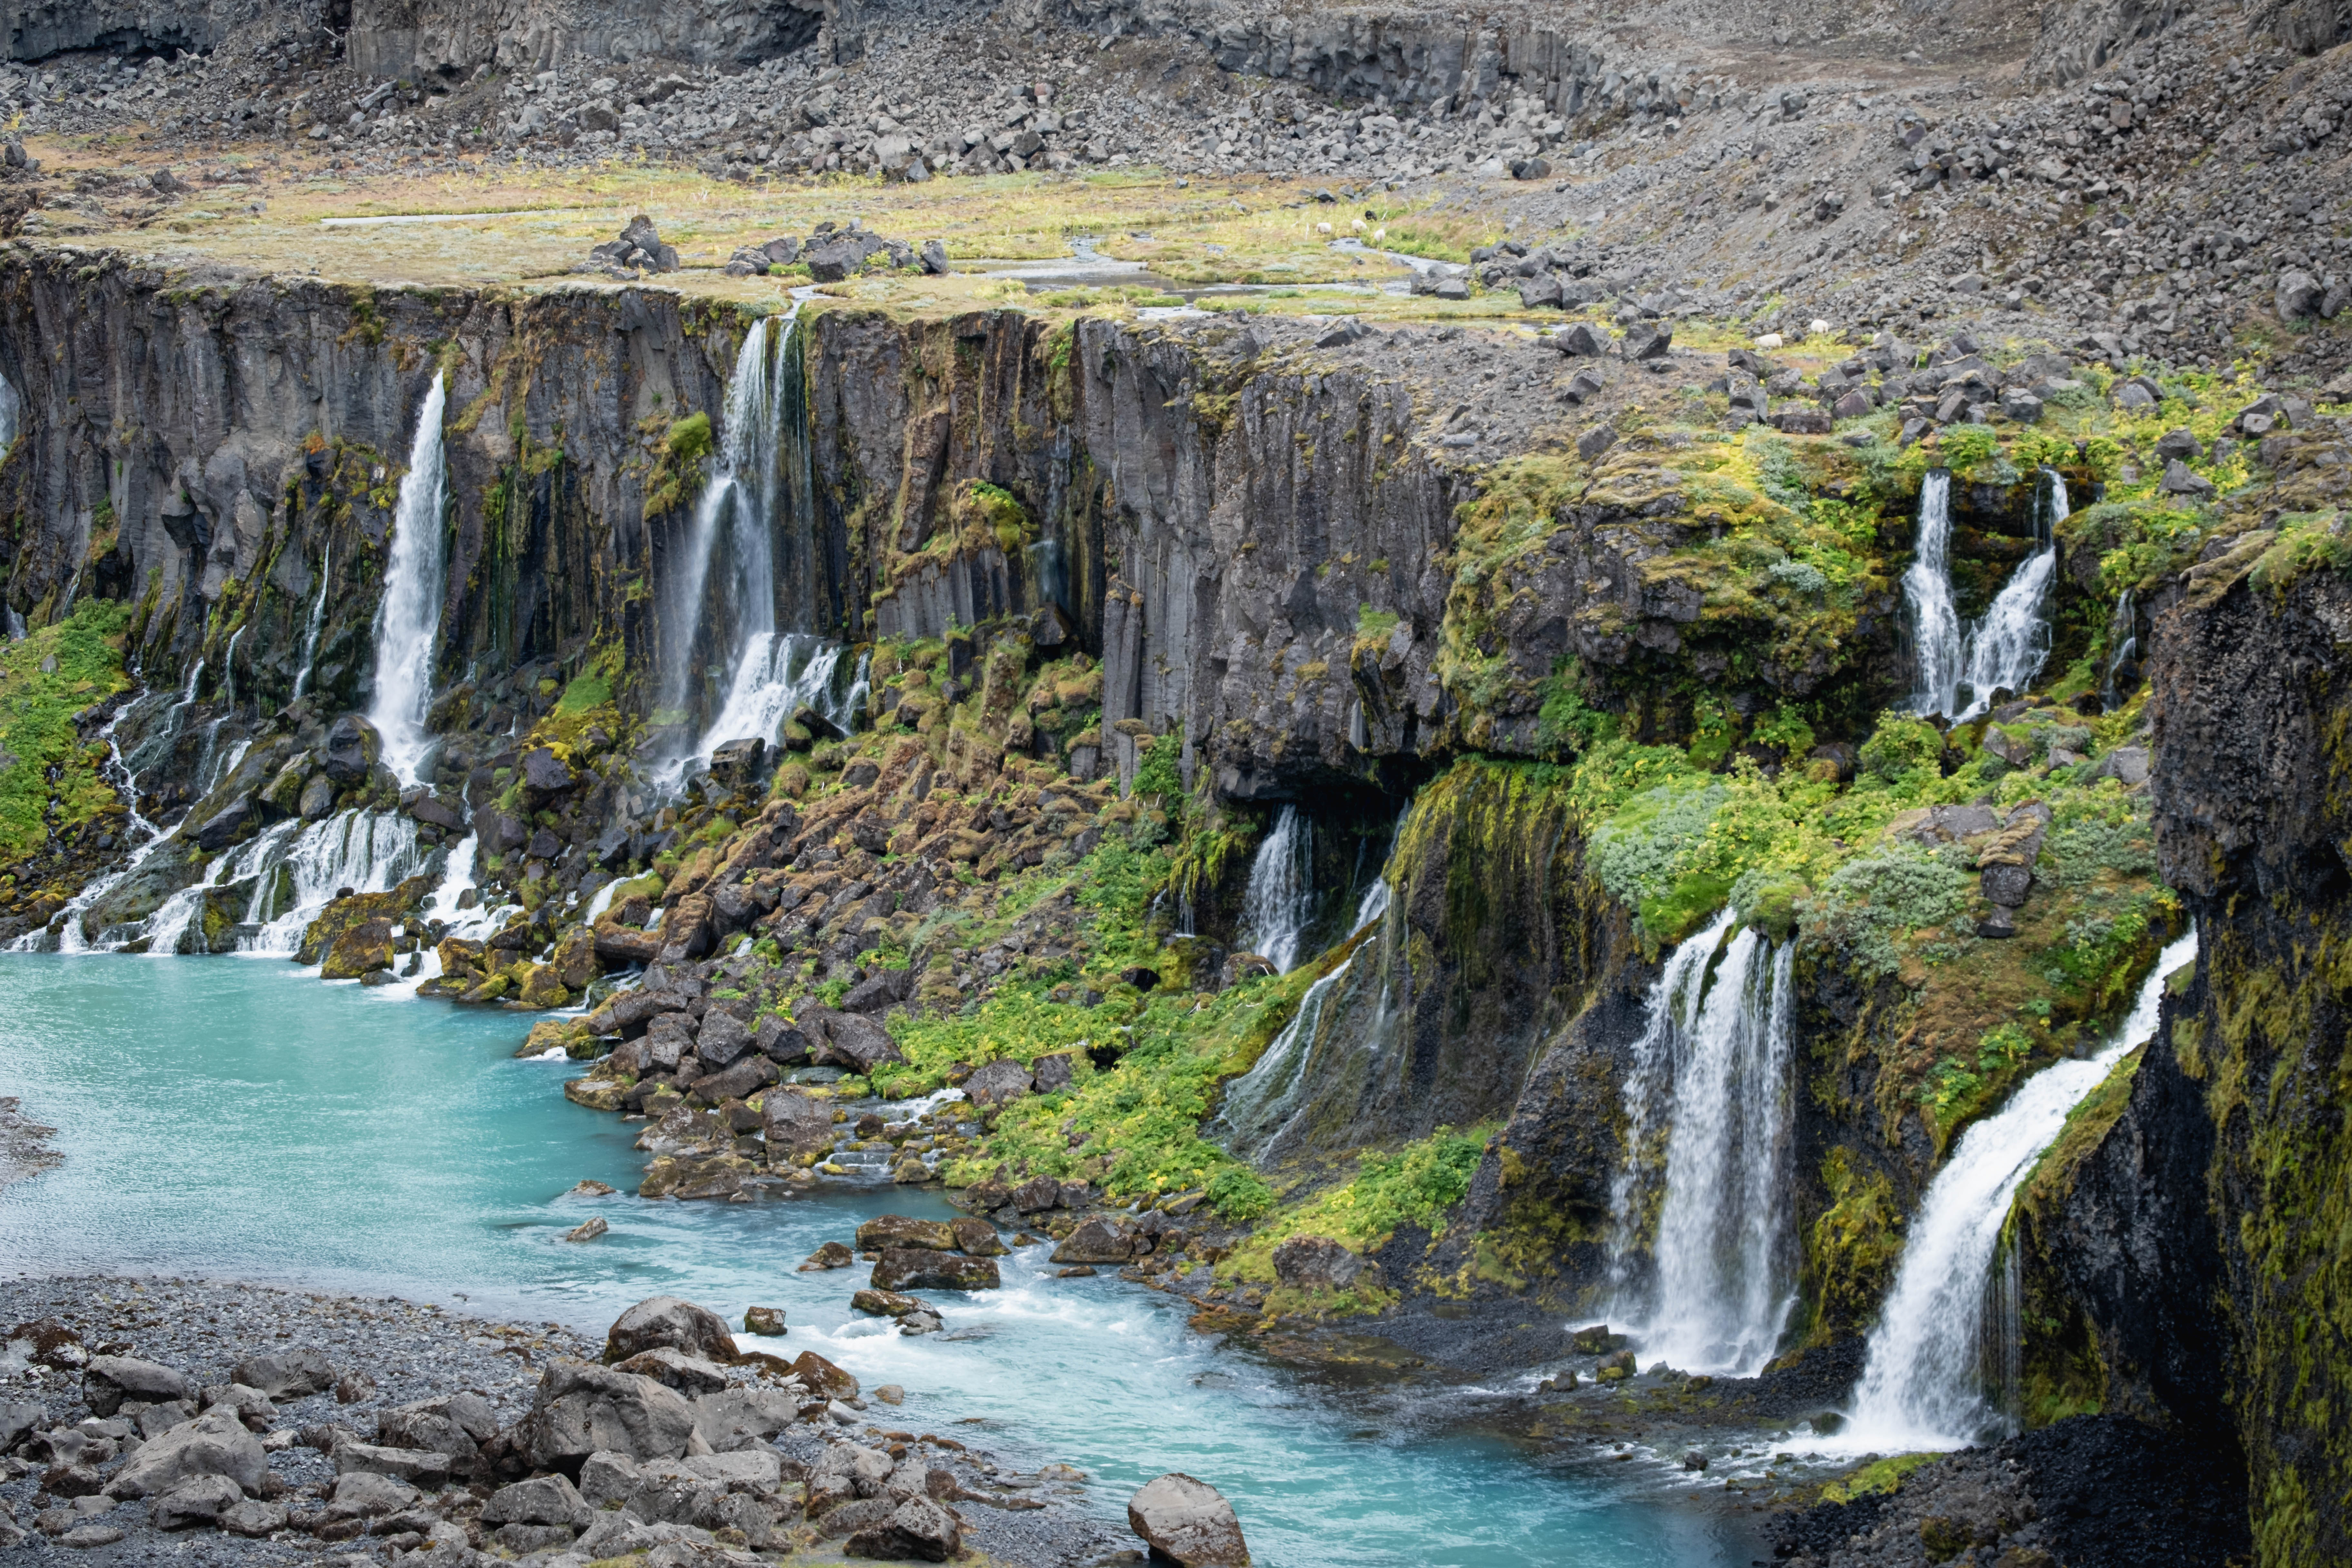
\includegraphics[width=0.3\textwidth]{fotos/b}
  \caption{Noch ein Bär}
\end{figure}

\lipsum[1-4]